%%%%%%%%%%%%%%%%%%%%%%%%%%%%%%%%%%%%%%%%%%%%%%%%%%%%%%%%%%%%%%%%%%%%%%%%%%%%%%%
%
% 
% 
%%%%%%%%%%%%%%%%%%%%%%%%%%%%%%%%%%%%%%%%%%%%%%%%%%%%%%%%%%%%%%%%%%%%%%%%%%%%%%%


\chapter{Simulation Method}
\label{sec:Simulation Method}

\section{FEM}


\section{Simulation Setup}
\subsection{Sphere vs Rigid Plane}
In this simulation the collision of two viscoelastic spheres is studied. Both the spheres have the same magnitude of velocity but opposite directions. Therefore to simplify the model and computation, instead of simulation two spheres colliding, a single sphere colliding against a rigid plane can be simulated. This setup would be equivalent to the original problem as both the spheres are the same in all aspects except for having different directions of velocities.

\subsection{Symmetry}
To further simplify the model, instead of considering the complete sphere, only a 2D semi-circular cross-section is considered. As the spheres are symmetric about the central rotational axis and the angle of contact is 90 degrees, there would not be any velocity in the Y direction. 

\subsection{Mesh}

\begin{figure}
    \centering
	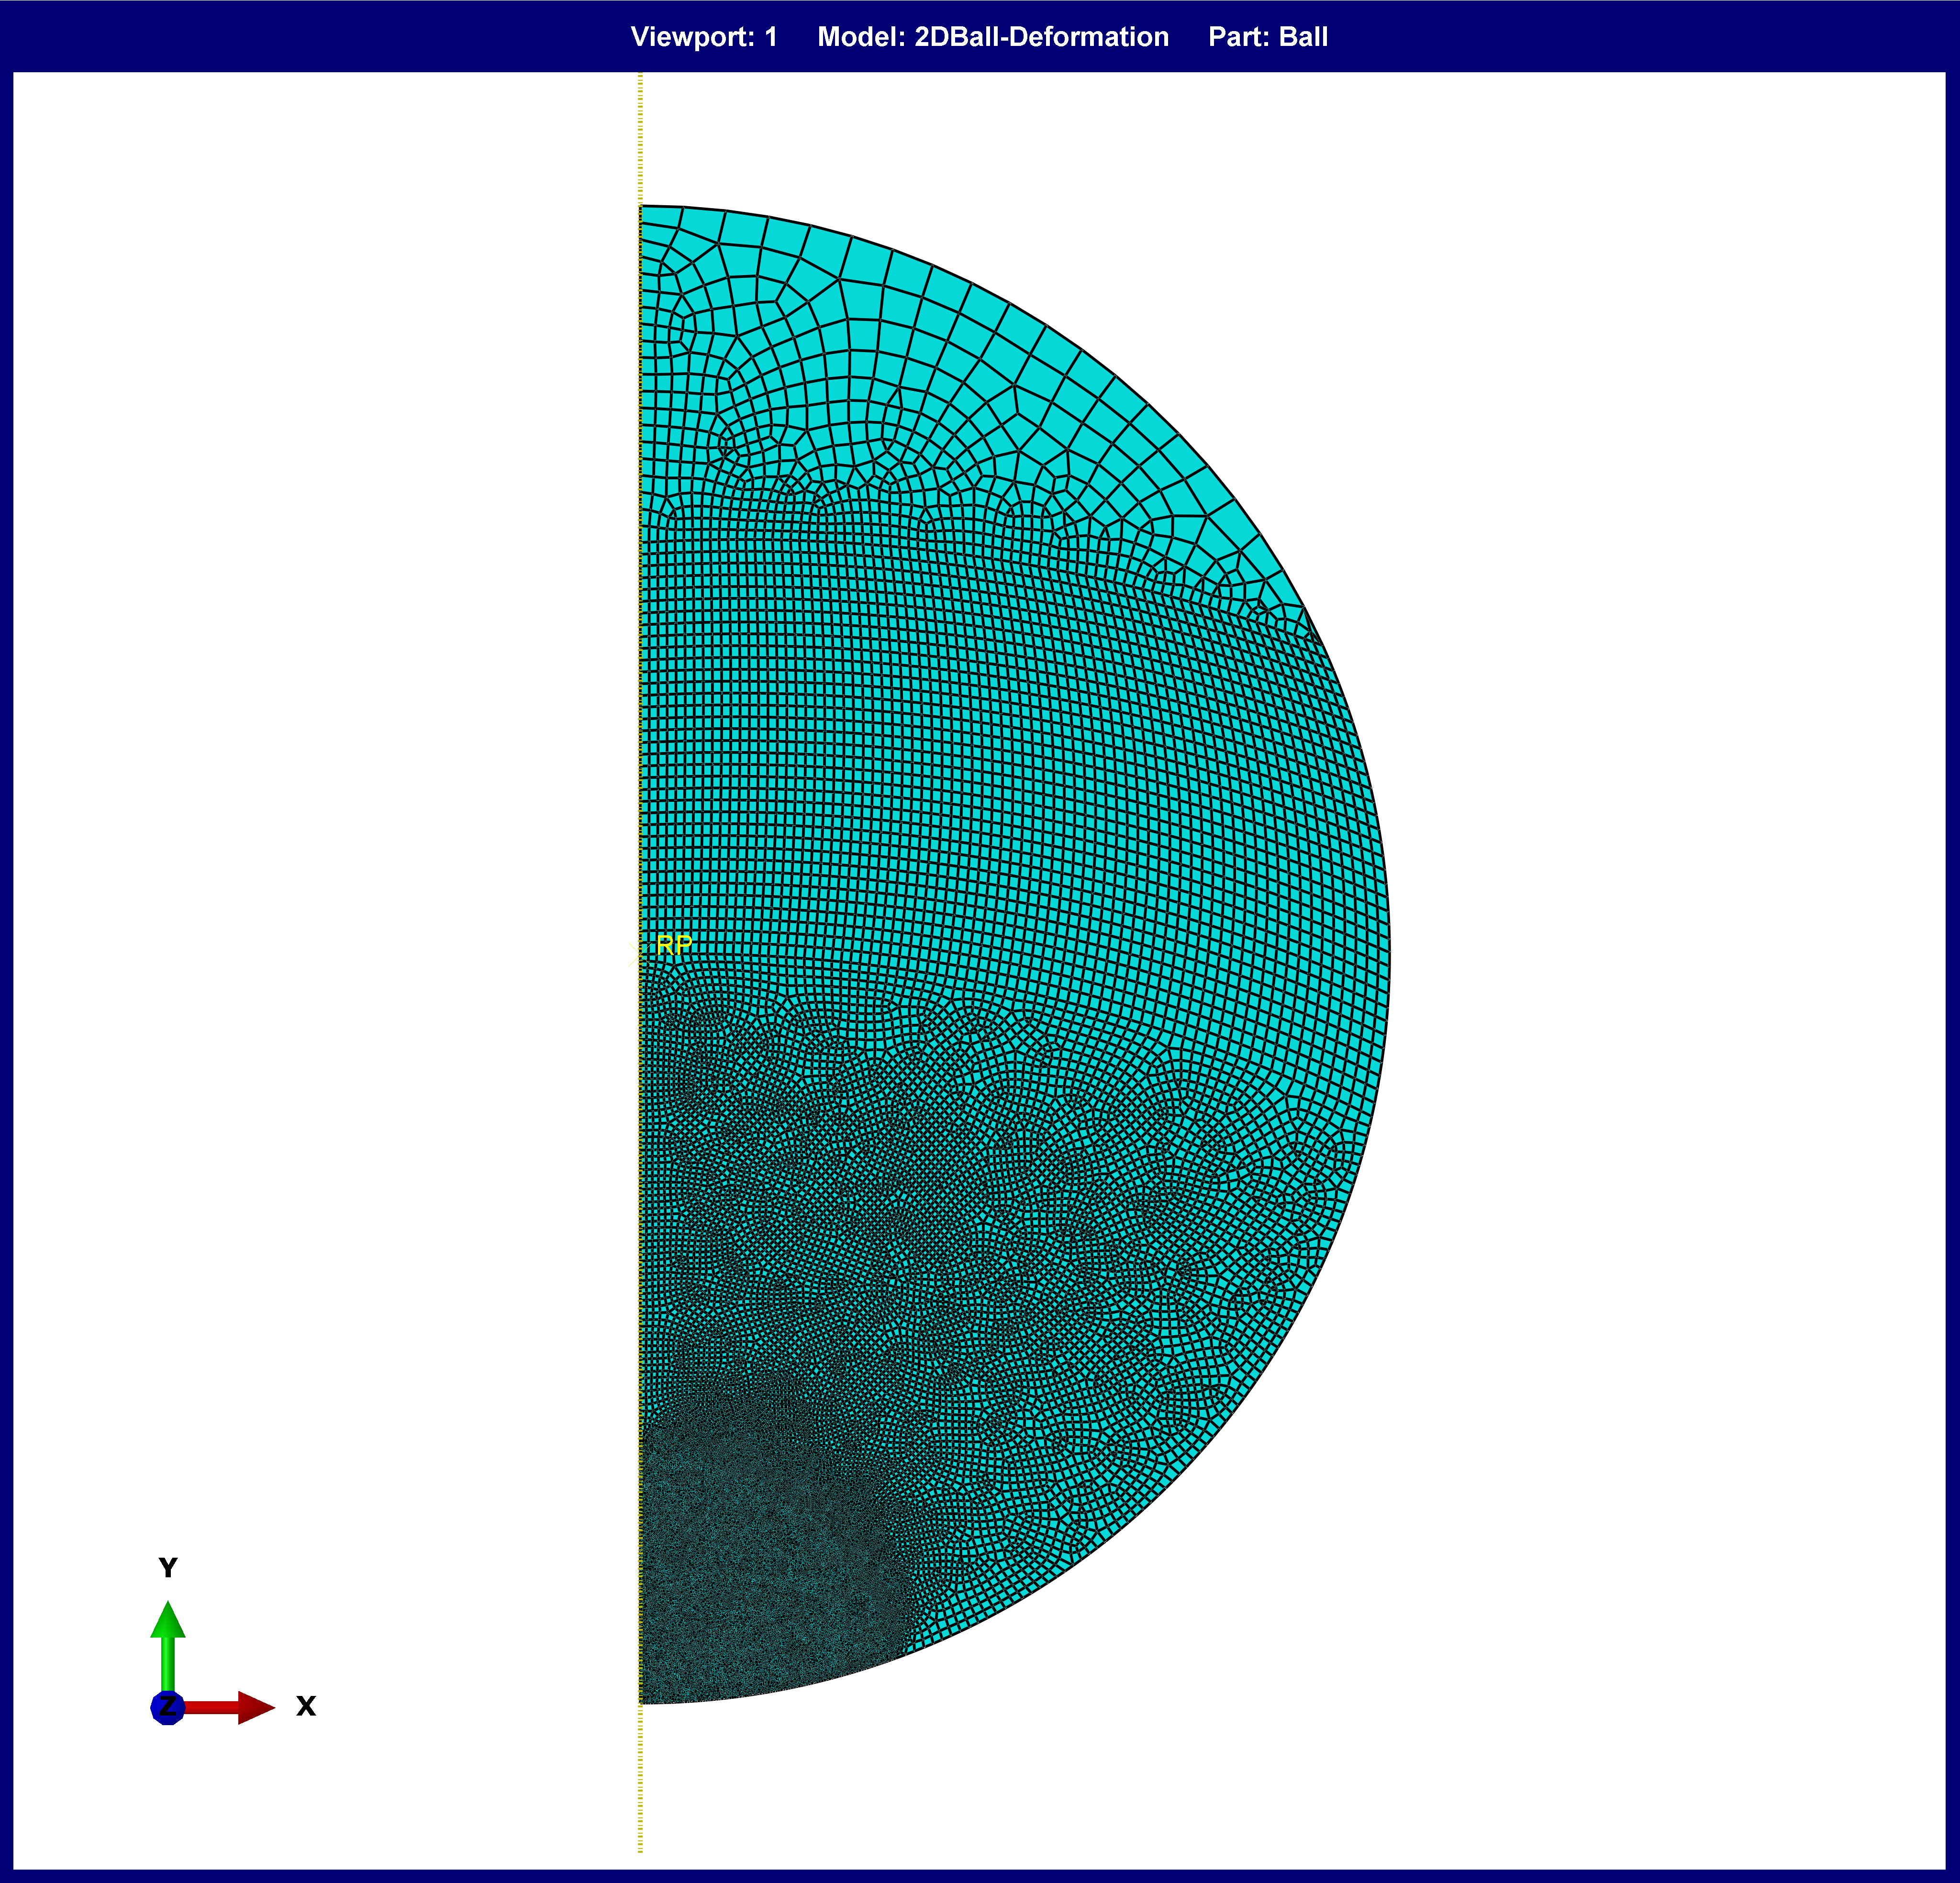
\includegraphics[scale=0.075]{../images/Mesh/Mesh.png}
	\caption{Mesh}
	\label{fig:mesh}
\end{figure}

The \ref{fig:mesh} shows the mesh used in the simulation. We can see that the mesh is finer at the bottom of the sphere as it is the point of contact and would undergo massive deformation during the impact. 

\begin{figure}
    \centering
	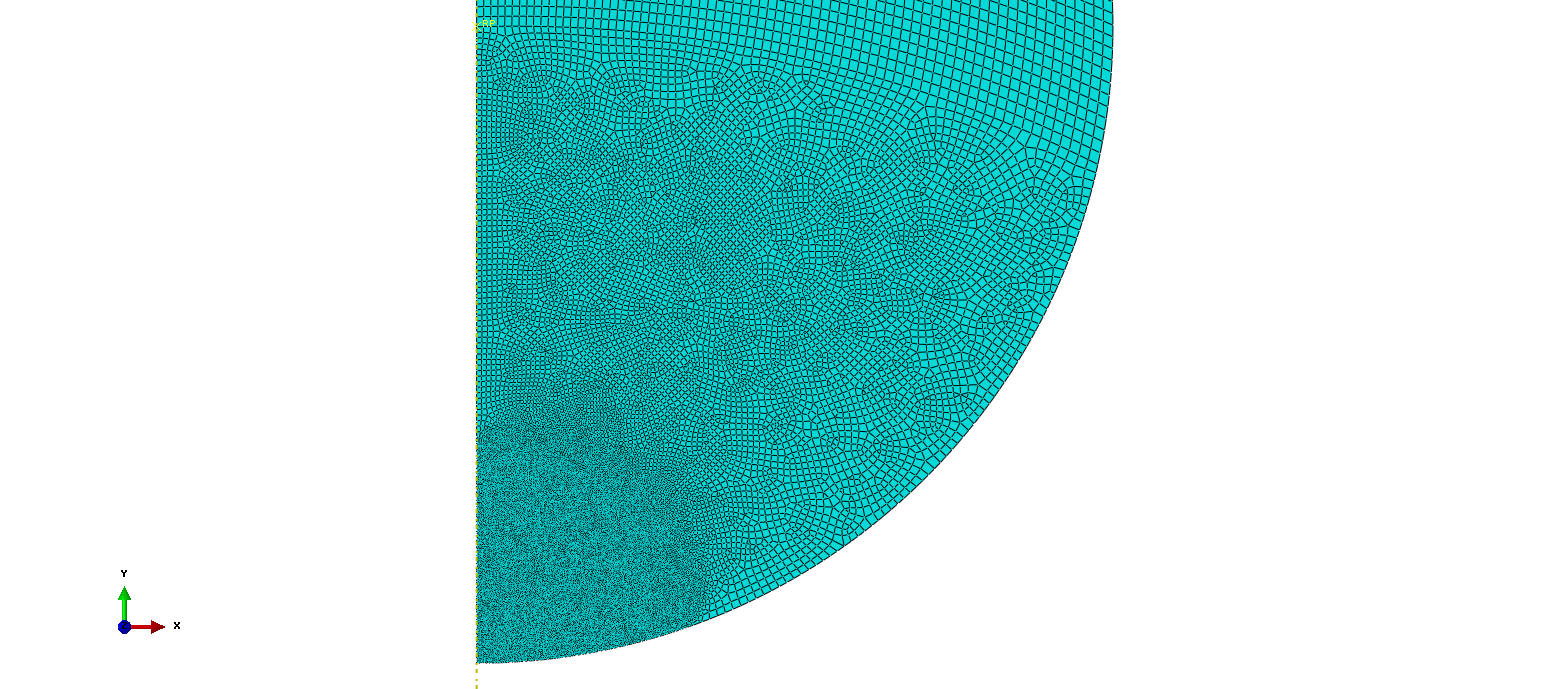
\includegraphics[scale=0.075]{../images/Mesh/Mesh_Bottom_Half_lowRes.png}
	\caption{Bottom Half of Mesh}
	\label{fig:mesh_bottom_half}
\end{figure}

The \ref{fig:mesh_bottom_half} shows an enlarged image of the bottom half of the mesh. We can see the degree of fineness of the mesh compared to the other half of the sphere.


\subsection{Rigid Plane}

The figure shows the rigid plane against which the sphere would be colliding. 

\section{Measurement Quantities}

\subsection{Displacement}

To measure the displacement of the body, the displacement of the center of mass was measured. The center of mass of the of a sphere is located at the sphere. The figure shows the center of the 2D semi-circle which was considered as the sphere of the model. To measure the displacement center of mass of the sphere, the displacement of center of the semicircle was considered.

\subsection{Kinetic Energy}

The kinetic energy of an object is the energy that it possesses due to its motion. As the aim of the thesis is to measure the co-efficient of restitution, which is directly related to the restitution kinetic energy in the body after the collision is completed.

\begin{equation}
Kinetic Energy(KE) = \frac{mv^{2}}{2}
\end{equation}
 
 where $m$ is the mass of the object and $v$ is the velocity of the object.

\subsection{Strain Energy}

The strain energy is the energy stored by a system undergoing deformation. During a collision, a part of the kinetic energy is converted into strain energy. This strain energy can also be observed as vibration on the body of the object. When the load is removed,

\begin{equation}
Strain Energy(U) = \frac{V\sigma\epsilon}{2}
\end{equation}

where $V$ is volume, $\sigma$ is stress and $\epsilon$ is strain.

\subsection{Co-efficient of Restitution}

The co-efficient of restitution describes the energy transfer 	 

\section{Verification}

To verify the correctness of the simulation setup, various meshes were tried. 
As Abaqus CAE has an option to automatically choose a suitable timestep, the automatic option was chosen.